\documentclass[a4paper,12pt]{article}
\usepackage{flafter,epsf}       
\usepackage{amsmath}
\usepackage{amsfonts,amsbsy,amssymb,bbm}
\usepackage{amsthm}  %% proof enviroment
\usepackage{natbibOrig}

\usepackage[pdftex,
colorlinks=true, %makes the links show up in color, rather than in a box
citecolor=black, %color of the in-text citation numbers
urlcolor=blue %color of the url links
]{hyperref}
\usepackage{wrapfig}
\bibliographystyle{unsrt}

%\usepackage[pdftex,
%colorlinks=true, %makes the links show up in color, rather than in a box
%citecolor=black, %color of the in-text citation numbers
%urlcolor=blue %color of the url links
%]{hyperref}

\sloppy 
\usepackage{graphicx}
%\bibliographystyle{natbib}

% Using the following to mark changes for review
\usepackage{color}
\definecolor{red}{rgb}{1,0,0}
\newcommand{\mc}[1]{\textcolor{red}{#1}}
%\newcommand{\mc}[1]{#1}   % Replace above line with this to eliminate all coloring

\input{epsf}

\newcommand{\peace} {{\small PEACE}}
\newcommand{\wcd} {{\small WCD}}
\newcommand{\capthree} {{\small Cap3}}
\newcommand{\easycluster} {{\small EasyCluster}}

\newcommand {\rel} {\mathbb{R}}
\newcommand {\com} {\mathbb{C}}
\newcommand {\nat} {\mathbb{N}}
\newcommand {\rat} {\mathbb{Q}}
\newcommand {\ganz} {\mathbb{Z}}
\newcommand {\indicator} {\mathbbm{1}}

\newtheorem{defi}{Definition}
\newtheorem{theo}{Theorem}
\newtheorem{corol}{Corollary}
\newtheorem{prop}{Proposition}
\newtheorem{example}{Example}
\newtheorem{lemma}{Lemma}
\newtheorem{problem}{Problem}[section]

\textheight 21cm
\textwidth 16cm
\oddsidemargin -0.1cm
\evensidemargin -0.1cm

\newlabel{sensitivityFig}{3}
\newlabel{seq_runtime}{4}
\newlabel{SangerReal}{1}


\begin{document}

\title{PEACE: {\underline P}arallel {\underline E}nvironment for {\underline A}ssembly
  and {\underline C}lustering of Gene {\underline E}xpression}

\date{}

\maketitle  

\begin{appendix}

\renewcommand{\theequation}{S\arabic{equation}}
\renewcommand{\thefigure}{S\arabic{figure}}
\renewcommand{\thetable}{S\arabic{table}}
\setcounter{equation}{0}

\section{Distance metrics, heuristics and filters}

\subsection{The distance metric}
$d^2$, as outlined by {\it Hide et al.} \cite{Hide94}, is an {\it
  alignment free} distance pseudo-metric which quantifies local
similarity between sequences based on a simple word count.  Let
$c_x(w)$ denote the number of times word $w$ occurs in string $x$.  We
search for similarity between strings $x$ and $y$ by looking at the
difference between $c_x(w)$ and $c_y(w)$ for different words $w$.
Specifically,  for all words of a fixed length $k$, we calculate:
\begin{equation*}
d^2_k(x,y) = \sum_{|w|=k}(c_x(w) - c_y(w))^2
\end{equation*}
However, applying such a definition to two sequences as a whole leads
to a measure of global similarity, while we want to measure local
similarity (thus, for example, assigning two sequences with
sufficiently long overlapping ends to be at a distance of zero -- or a
small distance if errors are present).  For this, instead of comparing
the entire two strings, we compare sliding windows from each string of a fixed
size $r$.  Formally, for sequences $x$ and $y$ ($|x| \geq r$, $|y|
\geq r$), we define:
\begin{equation}
\label{d2def}
d^2(x,y) = 
\min\left\{d^2(u,v) \; : \; u \sqsubseteq x, v \sqsubseteq y, |u|=|v|=r\right\}
\end{equation}
(where $u \sqsubseteq x$ denotes that $u$ is a substring of $x$).
Defined as such, $d^2$ is, in a mathematical sense, a {\it
  pseudo-metric}: $d^2(x,y) = 0$ does not imply $x=y$.

The \textsc{peace} implementation of $d^2$ was initially based on the description from
{\it Hazelhurst} \cite{Hazelhurst04}.  For parameters
we adapted those used by the \textsc{wcd} clustering tool \cite{Hazelhurst08a}:
a word size $k=6$ and a window size $r=100$.

\subsection{Improved Distance Matrix}
Our ``two-pass $d^2$'' algorithm works by sampling a subset of window
pairs evenly distributed across the sequences, narrowing down a
smaller region in which to search for the best scoring window-pair.
In the first pass, the algorithm look at every length $r$ window on one sequence,
but on the other sequence we skip the window by $s$ bases between
every sampling.  It then take the best such window pair, extend
each of these two windows by $s$ bases in each direction, and apply
(\ref{d2def}) to this limited region.

In \textsc{peace}, we use $k=6$, $r=100$, and $s=50$.

\subsection{Filtering heuristics}
\textsc{peace} uses the $u/v$ and $t/v$ heuristics, roughly as described by {\it
  Hazelhurst et al.} \cite{Hazelhurst08a} as filters that allows us to avoid
over 99\% of the potential $d^2$ calculations.  Each heuristic takes two
sequences and estimates whether it is worth proceeding to the $d^2$
computation by sampling and comparing word frequency across the two
sequences.  The $u/v$ heuristic looks at every $h$-th word of size $v$
on one sequence, and rejects if it does not find at least $u$ occurrences
of these words on the other sequence.  The $t/v$ heuristic demands
that there be at least $t$ size $v$ words on one sequence that occur
within a $l$ base range within the second sequence.  If a sequence
pair meets the requirements of both these filters, then we compute the
$d^2$ distance.

In \textsc{peace}, we set $h=16$, $v=8$, $u=4$, $t=65$, and $l=100$.

\section{MST-Based  Calculations}

While $d^2$ serves to quantify sequence distance, the basis for the
clustering algorithm is the minimum spanning tree (MST).  Viewing the
ESTs as nodes and the data set as an $d^2$-weighted graph, the
derivation of a minimum spanning tree results in the placement of
nodes of a given tree into a restricted neighborhood of the graph.  By
then removing larger edges, we are left with connected components
corresponding to the gene-based clusters.  The MST-based clustering
method has been used effectively in other applications, but to our
knowledge this is the first such use for the  EST
clustering problem \cite{Jain99,Wan08}.

\subsection{Calculation of the MST}

To calculate this MST we use Prim's algorithm \cite{Prim57}.  For a
graph of $n$ nodes and $e$ edges, Prim's can be implemented such that
the algorithm has an $O(e + n \log n)$ worst-case runtime.  However,
the {\it narrow-band} nature of the model allows us to reduce this
bound.  If we were to model only the edges connecting adjacent nodes,
we would find the node degrees to be very small relative to $n$: any
EST overlaps only a few others, and has no connection to a vast
majority of the data set members.  Since we can quickly eliminate most
of these excess edges with the $u/v$ and $t/v$ heuristics (removing
more than 99\% of all edges before applying Prim's), we find in
practice that $e$ is a very small fraction of $n^2$.  In the
runtime results (Figure~4), we find that when holding the EST size
distribution constant, the tool as a whole has a runtime of $O(n^2)$
-- appearing to dominated by the time required to apply
the filtering heuristics to every EST pair.

\subsection{Removing edges}

Once the MST is has been calculated, our last step is to remove all
edges exceeding a threshold weight $T$, taking the resulting
components as our clusters.  \textsc{wcd}, when faced with a similar
challenge, sets the threshold at $T=40$, hypothesizing that EST pairs
with a $d^2$ distance of greater than 40 are unlikely to overlap.  \mc{We
have set our threshold to the same $T=40$ (with discussion below on
the effects of changing this).}

\section{Adaptive $d^2$}

\mc{In the above discussion of $d^2$ we assume sequences of at least 100
bp, and in practice use a window of size 100.  While the technique
should be, in principle, adaptable to short-read sequences (decreasing
window size as necessary), there are some problems in the details.
Diminishing window sizes implies both diminishing accuracy (requiring
the threshold be adjusted) and increasing runtime (as there are
potentially more window pairs).  More importantly, there is the
problem of non-homogeneous sequence lengths: short-read technologies
tend to produce short reads, but some technologies can still include
long reads in their output.  Hence it is not immediately clear how to
compare a very short read against a very long one.}

\mc{We address these issues with our {\it adaptive $d^2$} strategy that
works as follows: we partition sequences by length into disjoint groups.  For each
group we pick a constant window size and threshold tailored to the
length range of the group (as well as filtering heuristic constants),
and use those values when computing the $d^2$ distance for two
sequences in the same group.  We do not compute distances between
sequences in non-adjacent groups (i.e. a member of the ``shortest
groups'' against a member of the ``longest groups'' if there is an
intervening sized group).  Once computed, we assign to the MST
edge the ratio of the $d^2$ score to the group threshold, thus
normalizing the weight for comparisons ``between groups'' and
effectively giving us an edge-removal threshold of 1.}

\mc{By restricting $d^2$ comparisons to within a group, we minimize the
effects of the heterogeneous sequences lengths by restricting our
comparisons to only sequences of similar lengths.  By not restricting
ourselves to a single window size, we allow ourselves to, when possible, avoid the
performance hit of using a small window.  As we are not comparing
sequences from different groups we bypass the question of how to
compare a long sequence against a short one.  And because the
groups overlap in content, we still get implicit comparisons between
long and short sequences in terms of the resulting path of the minimum
spanning tree that makes use of these ``linking'' nodes.}

\mc{In the \textsc{peace} implementation, we subdivide into three groups:
\begin{itemize}
\item Less than 150 ($w=50$, $T=40$, $t=20$, $u=4$).
\item Between 150 and 400 ($w=75$, $T=60$, $t=35$, $u=6$)
\item Greater than 400 ($w=100$, $T=80$, $t=50$, $t=50$).
\end{itemize}}




\section{Simulated Test Results}

In {\it Hazelhurst et al.} \cite{Hazelhurst08a} the authors conduct
an investigation of \textsc{wcd} \mc{(version 0.5.1)} against a number of clustering
tools.  As they make a convincing argument that \textsc{wcd} is returning
better results then the tools against which they compare, we limit our
analysis to a comparison of \textsc{peace} against \textsc{wcd} and the \textsc{cap3} assembly
tool \cite{Huang99} -- a tool which implicitly clusters while
performing assembly.  We do so by applying all three tools to a number
of data sets, both simulated and real.

\subsection{Simulation Tool and Parameters}

For simulated data sets we use the {\bf ESTsim} tool to generate
simulated EST data sets \cite{Hazelhurst03}, using the collection of
zebra fish genes that served as a basis for the \textsc{wcd} simulations
\cite{Hazelhurst08a}.  In generating the ESTs, ESTsim models three
types of error (general base read errors, errors due to
polymerase decay, and primer interference), and allows those errors to
take the form of substitutions, deletions, and insertions (of bases
and Ns).  See the paper for a discussion of the probability
distributions and default parameters.  For generating our simulated
data, we use the default values for all parameters that are not
explicitly being subjected to variation in our experiments --
paralleling the testing of the \textsc{wcd} tool.



\subsection{Methodology} 

Each estimate given in the main paper, or in the following, is
averaged over 30 trials.  Each trial consists of the application of
all three tools to a simulated data set, the set having been derived
from the application of the ESTsim tool to a set of 100 zebra fish
gene sequences \cite{Hazelhurst03}.  All confidence intervals are
calculated at a 95\% level of significance.

\subsection{Result Quality}

\mc{Our primary measurement tools if measurement are sensitivity, the
Jaccard Index, Type 1 error and Type 2 error
(Figure~3).  Sensitivity is the ratio for true
positives to actual positives ($tp / (tp + fn)$) -- the fraction of
sequences from the same transcript that are identified as such.  The
{\it Jaccard} index combines both sensitivity and specificity,
calculated as the ratio of true positives to the sum of true
positives, true negatives, and false positives ($tp / (tp+fn+fp)$)
\cite{Hazelhurst08a}.  Notably, when we removed duplicated genes
before generating the simulated EST sets, we found all three tools to
have perfect specificity: no false positives.}

\mc{Type 1 and Type 2 errors, as defined in {\it Wang et al.}
\cite{Wang04}, measure quality at the level of the genes from which
the ESTs were derived.  For Type 1 error, we look at the fraction of genes
that were broken into two or more partitions, while in
Type 2 error we look at the fraction of clusters that contain two or
more genes.}

\mc{A fifth metric is the number of singletons produce by a
  tool:  sequences that  could not  be  assigned to  any cluster.   In
  practice such a sequence could represent complete coverage of a very
  short transcript (one that may be otherwise had to identify), but is
  more likely to be an error in the clustering algorithm.  In order to
  identify  the first  it is  important  to minimize  the second.   In
  Figure~\ref{singletons} we look at the number of singletons produced
  by each tool when run on  simulated data in which there should be no
  singletons produced,  seeing a very slight improvement  of PEACE over
  WCD in certain error ranges.}

\begin{figure}[tbp]
\centerline{
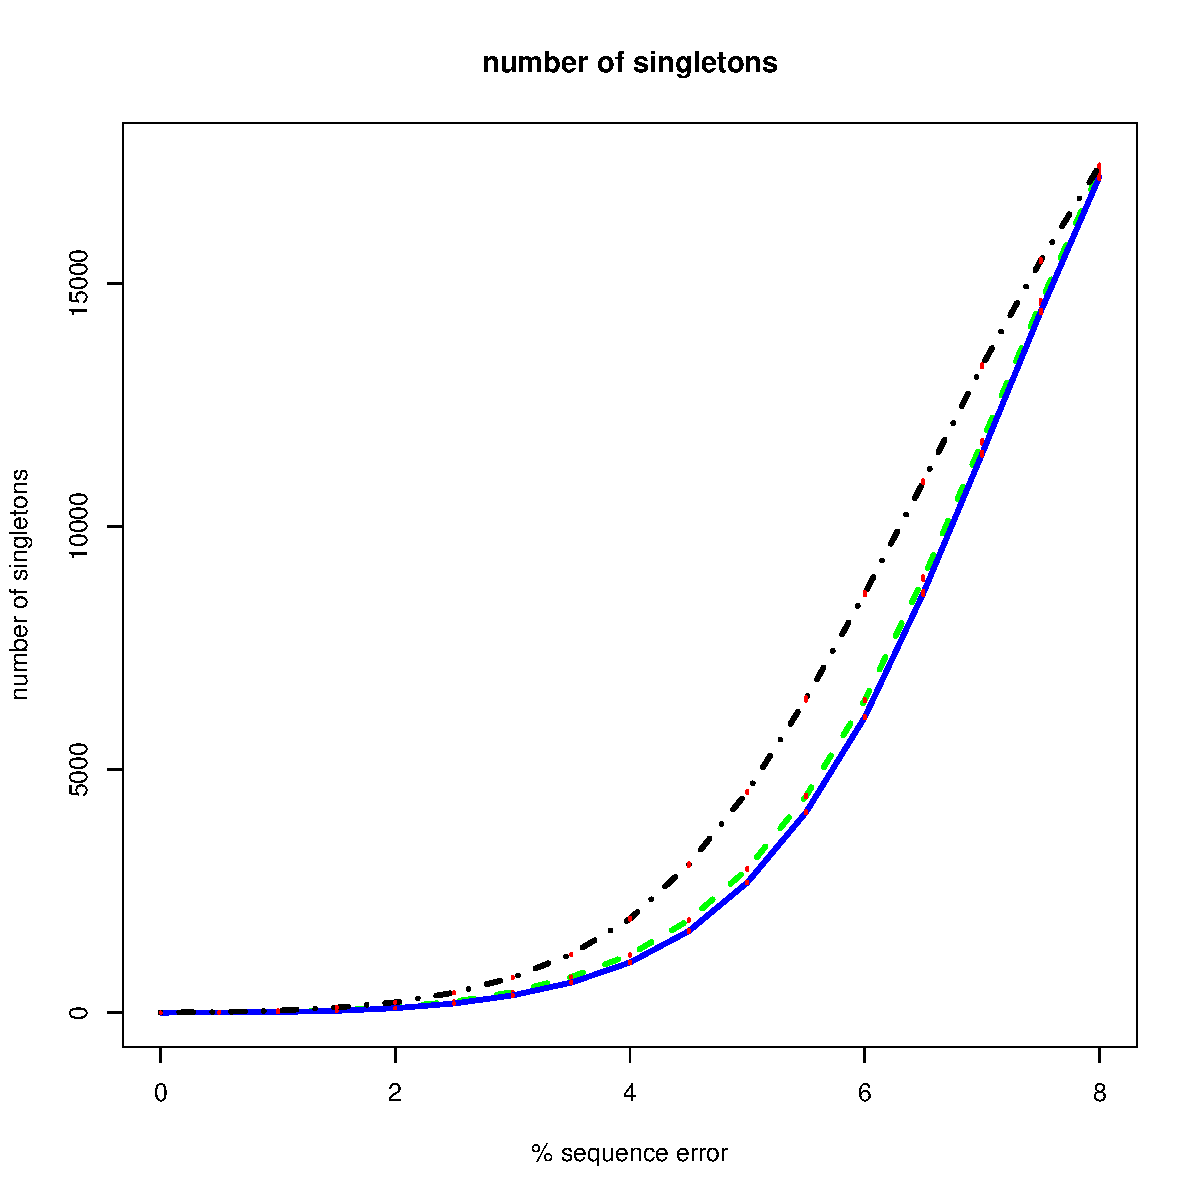
\includegraphics[scale=0.35]{pics.d/singletons_40.pdf}
}
\caption{Number of singletons produced by each tool in a simulated run
  where a fully correct clustering would have no singletons.  Values
  average over 30 trials.  Blue/Solid = \textsc{peace}, Green/Dashed =
  \textsc{wcd}, Black/Dot-Dashed = \textsc{cap3}.}\label{singletons}
\end{figure}


One of the difficulties in clustering EST data is dealing with
highly similar genes.  Genes with a high degree of similarity will
produce ESTs that reflect that similarity, hence appear to overlap --
resulting in the incorrect clustering of ESTs from separate genes.  Assembly tools
such as \textsc{cap3} may have more ability to discriminate between clusters
given their more intensive investigation of overlaps, but highly
similar sequences are going to cause a problem for any tool. 

In Figure~\ref{dups} we look at the ability of each tool to separate
duplicates as a function of the \% divergence between the
duplications.  Unsurprisingly, \textsc{cap3} (the assembler) does the best
here, able to effectively separate duplicates at $~92\%$ similarity
or less.  \textsc{peace} and \textsc{wcd} are roughly comparable, both clearly able to
separate duplicates out at a similarity level of $78\%$ -- but completely 
unable to distinguish sharing a similarity of $~88\%$ or more. 

\begin{figure}[tbp]
\centerline{
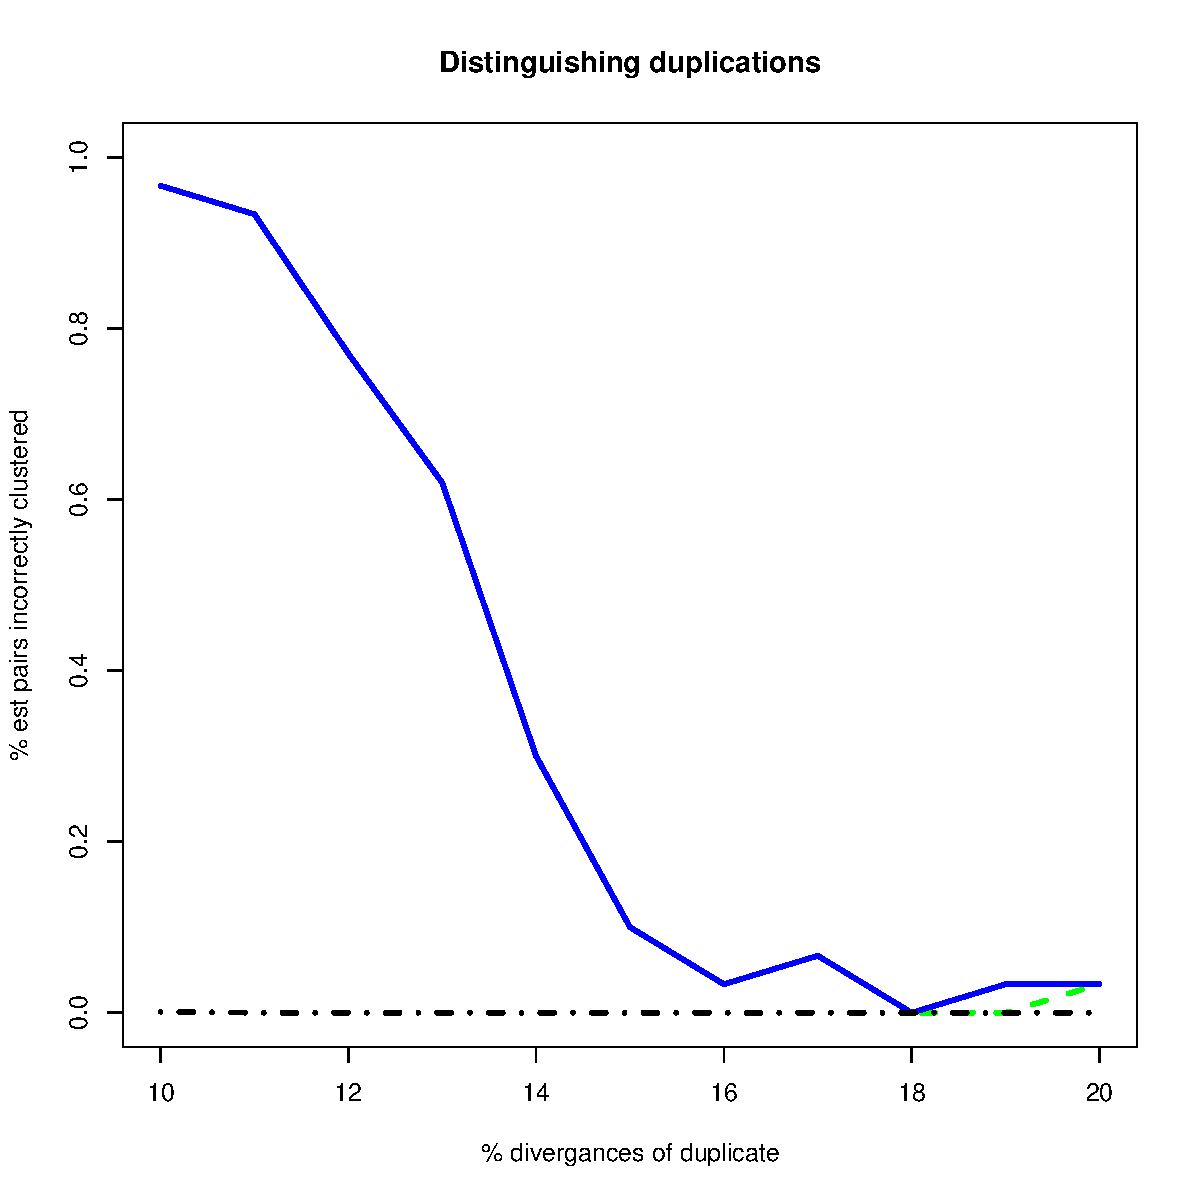
\includegraphics[scale=0.35]{pics.d/duplicates_40.pdf}
}
\caption{Ability to distinguish duplicates as a function of
  divergence.  Estimates averaged over 30 trials; one trial consists
  of taking a random gene, copying it and stochastically changing
  bases at the specified rate, then using the two genes as the bases
  for generating a simulated set. Blue/Solid = \peace, Green/Dashed =
  \wcd\/ (mostly obscured by the blue line), Black/Dot-Dashed =
  \capthree; variance was too small for visible plotting of
  confidence intervals.}\label{dups}
\end{figure}

\subsection{Raising the Threshold}
\label{sim_thresh}
\mc{ 
  The \wcd\/ tool uses a $d^2$ threshold of $40$ to determine whether
  two sequences are in the same cluster.  As this is equivalent to our
  $T$ threshold for dismissing MST edges, we have set it to the same
  default value when used for Sanger sequences.  However, we did
  experiment with higher values, to interesting results.  A basic
  analysis indicated that a $T$ value as high as 130 should not have a
  significant impact on its effectiveness as a discriminator.  And in
  fact this was born out in simulation, as shown in
  Figure~\label{SiJiT1T2130}.  In contrast with the equivalent results
  for a threshold of $T=40$, as shown in the manuscript, we see
  considerable improvement in \peace\/ over \wcd\/ in all metrics
  except Type 2 error, in which \wcd\/ slightly
  better. Unsurprisingly, this also makes a significant difference in
  the tool's ability to distinguish duplications: we see fairly poor
  performance in Figure~\ref{dups130}.  
}

\mc{
  Most importantly, while the higher threshold appeared to be better
  in theory and in analysis, it did not hold in practice.  In
  Table~\ref{SangerReal130} we show the match to the manuscript
  Table~1, and observe the poor performance of
  \peace\/ when looking at the Jaccard index.  It is clear that in the
  real data, the level of similarity is considerably higher then in the
  simulations, thus making the reduced specificity of the higher
  threshold considerably more of a problem.
}


\begin{figure}
  \centerline{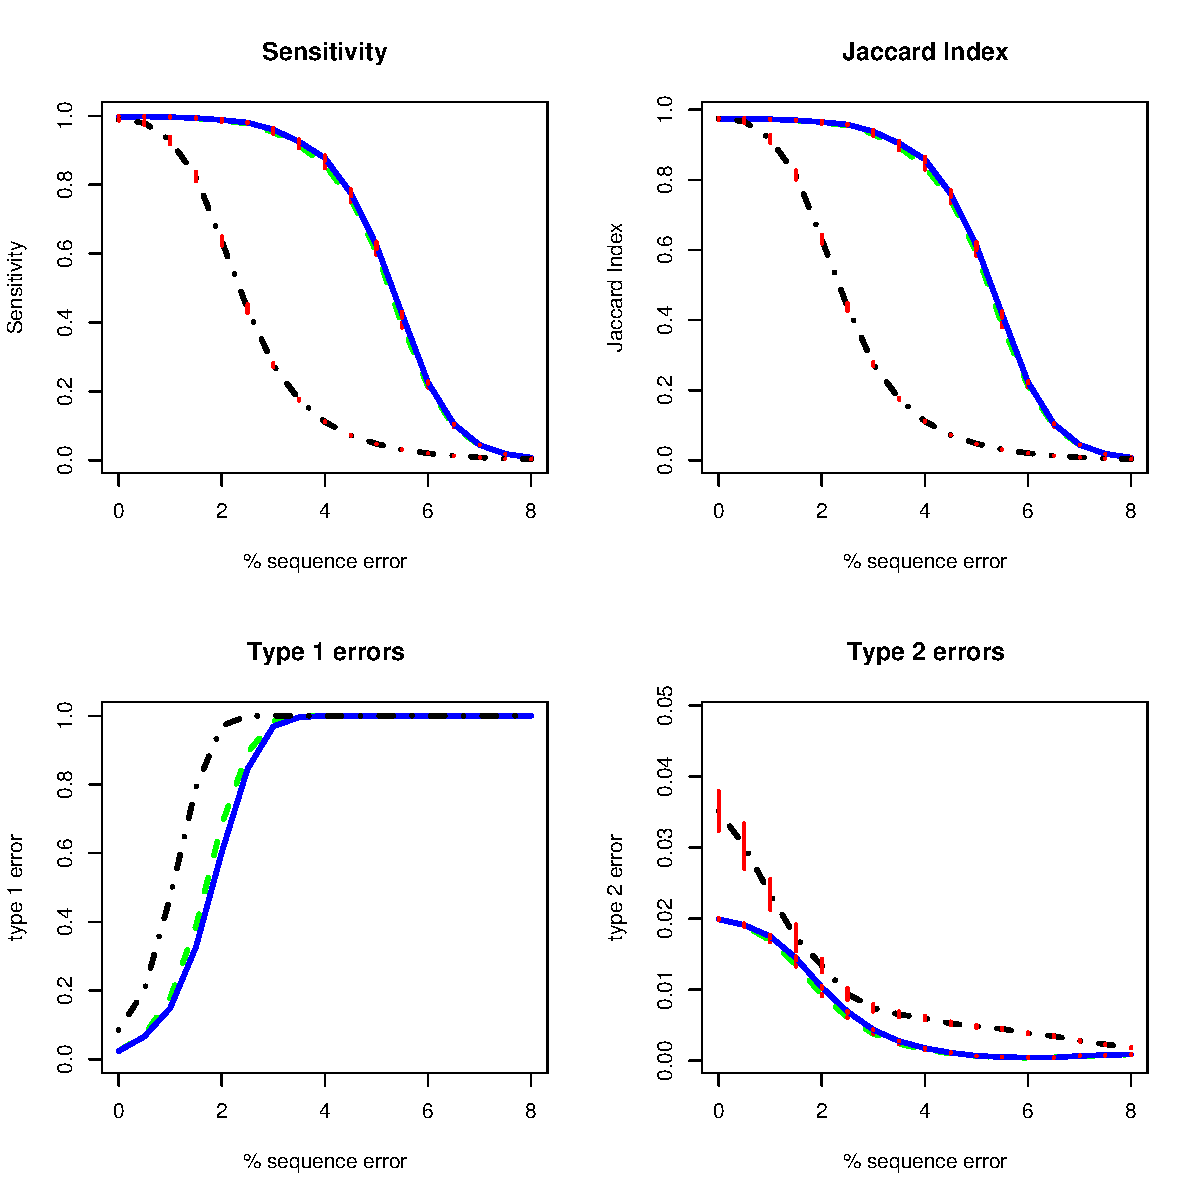
\includegraphics[width=3.35in]{pics.d/SeJiT1T2x40.pdf}}
  \caption{Comparisons of Sensitivity, Jaccard Index, Type 1 error and
    Type 1 error, based on the
    average over 30 simulated Sanger Sequence ESTs sets derived from 100 zebra
    fish genes  (see
    Supplementary Materials, Section C, for more details).  Blue/Solid
    = \peace, Green/Dash = \wcd, Black/Dot-Dash = \capthree; vertical
    tics = 95\% confidence intervals on estimates.  Intervals are not
    presented for Type 1 error due to the effective lack of
    variance.}\label{SeJiT1T2130}
\end{figure}

\begin{figure}[tbp]
\centerline{
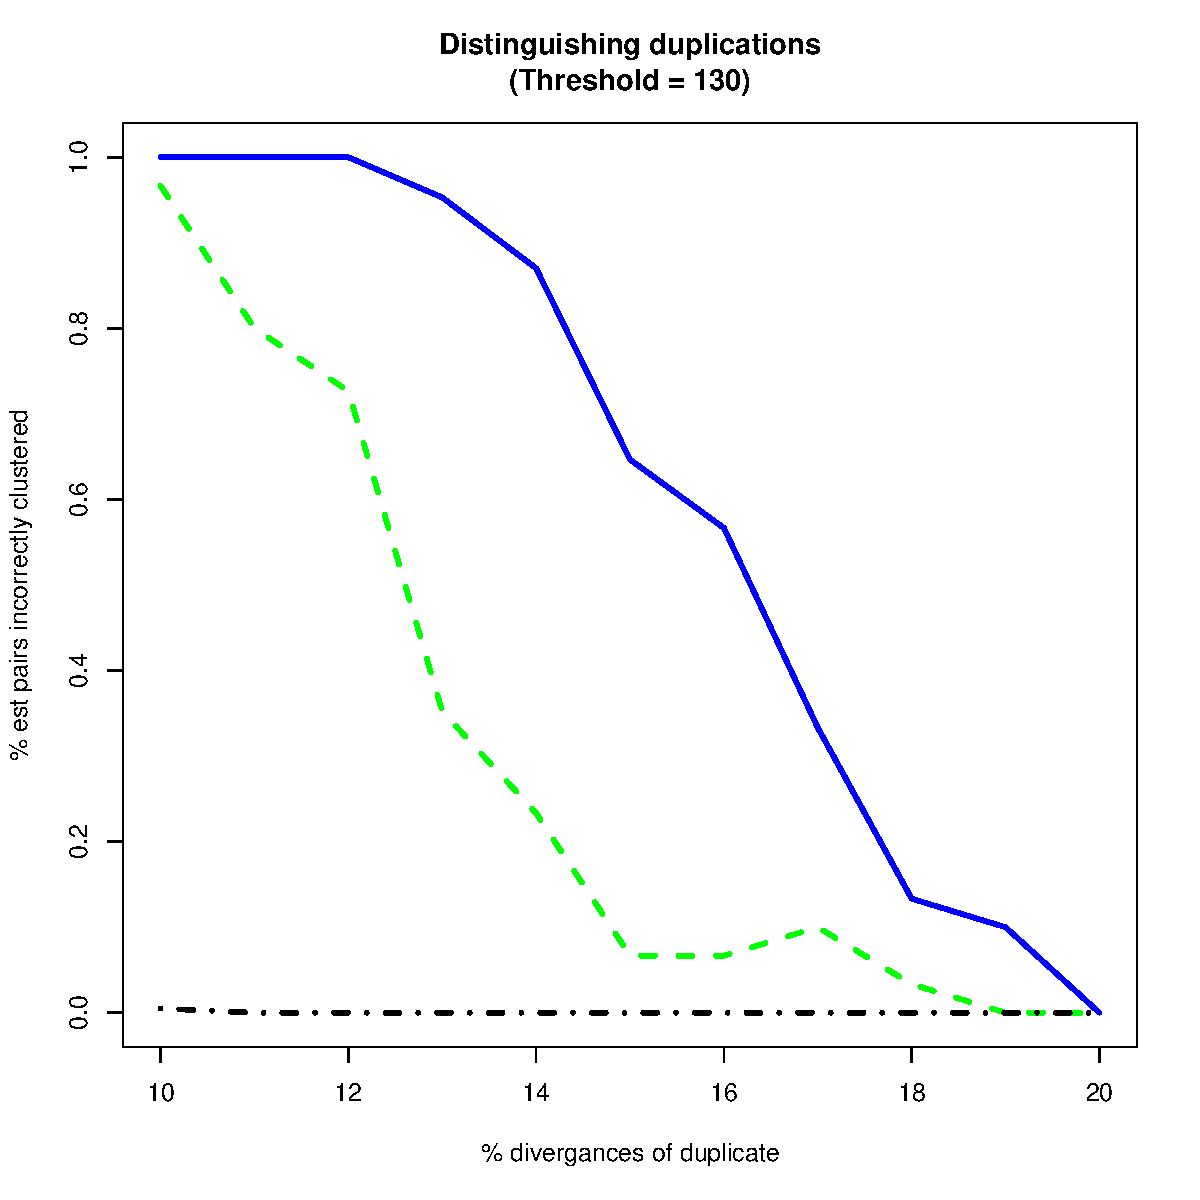
\includegraphics[scale=0.35]{pics.d/duplicates_130.pdf}
}
\caption{Ability to distinguish duplicates as a function of
  divergence.  Estimates averaged over 30 trials; one trial consists
  of taking a random gene, copying it and stochastically changing bases
  at the specified rate, then using the two genes as the bases for
  generating a simulated set. Blue/Solid = \textsc{peace}, Green/Dashed = \textsc{wcd}, Black/Dot-Dashed = \textsc{cap3};
  variance was too small for visible plotting of
  confidence intervals.}\label{dups130}
\end{figure}


\section{Real Data}

\subsection{Runtimes}

In Table~\ref{RunTime} we show the runtime of \peace\/ and \wcd\/ on
five different benchmark sets obtained from the WCD and EasyCluster
studies \cite{Hazelhurst08a,Picardi09}. 

\begin{table}[tbp]
\begin{center}
\begin{tabular} {|c|| c | c || c | c |}
\hline
 Benchmark & \begin{tabular}{c} Number of \\ Sequences \end{tabular}
 & \begin{tabular}{c} Number of \\ Bases \end{tabular} & Peace Runtme (s)&
 WCD Runtime (s) \\
\hline
\hline
 Human Cluster & 17733 & 11.7 Mb & 293 & 804 \\
\hline
 Cotton & 29,995 & 17.1 Mb & 222 & 339 \\
\hline
 Ricinus & 57,690 & 40.9 Mb & 1344 & 2356 \\
\hline
 A076941 & 76,941 & 32.8 Mb & 1166 & 966 \\
\hline
\hline
 A686903 & 686,904 & 294.7 Mb & 9449 & 2481 \\
\hline
\end{tabular}
\end{center}
\caption{Runtime for \peace\/ and \wcd\/ on benchmarks from the
  WCD and EasyCluster studies \cite{Hazelhurst08a, Picardi09}.
  Runtimes for the first four sets are sequential, while that last was
  run over thirty processors.}\label{RunTime}
\end{table}

\subsection{Higher Threshold}

\mc{ In Table~\ref{SangerReal130} we see the effect on the application
  of \peace\/ to the data sets from Table~1 when
  raising the threshold $T$ to 130 (see previous discussion in
  Section~\ref{sim_thresh}).  While doing this appeared to be fairly
  effective in simulation, it did not hold up in practice.  We see
  essentially no change in the sensitivity, but significant changes in
  the Jaccard Index (and a corresponding decrease in the total number
  of clusters).  We suspect that this is due to a higher number of
  more closely related genes than are present in the simulated
  data. Regardless, without considerably more investigation, these
  results indicated we should be leaving $T$ at a default rate of 40.
}

\begin{table}[tbp]
\begin{center}
\begin{tiny}
\begin{tabular} {| c || c || c | c | c | c | c | c | c |}
\hline
 & 
& Sensitivity & Jaccard & \begin{tabular}{c} Type 1 \\
  error \end{tabular} & \begin{tabular}{c} Type 2 \\
  error \end{tabular} &
\begin{tabular}{c} Number \\ of  \\
    Clusters \end{tabular} & \begin{tabular}{c} Number \\ of \\
    Singletons \end{tabular}
    & \begin{tabular}{c} Single \\ processor \\ runtime
      (s) \end{tabular} \\
\hline
\hline EasyCluster Human & PEACE & 0.999 & 0.106 & 0.027 & 0.030 & 67 & 2 & 295 \\
\cline{2-9} Benchmark & WCD & 0.998 & 0.672 & 0.144 & 0.044 & 113 & 16 & 804 \\
\cline{2-9} (111 Genes) & Cap3 & 0.657 & 0.643 & 1.000 & 0.001 & 2269 & 1827 & \mbox{NA} \\
\hline
\hline WCD A076941 & PEACE & 0.937 & 0.345 & 0.337 & 0.0342 & 18256 & 8135 & 1293 \\
\cline{2-9} Benchmark & WCD & 0.933 & 0.476 & 0.350 &  0.027 & 18787 & 8553 & 966 \\
\cline{2-9} (13240 genes) & Cap3 & 0.826 & 0.802 & 0.486 & 0.014 & 25042 & 14916 &
\mbox{NA} \\
\hline
\end{tabular}
\end{tiny}
\end{center}
\caption{Comparisons of runs on the EasyCluster human Benchmark
  Dataset and the WCD A076941 Arabidopsis thaliana dataset using the
  standard quality measurements with $T=130$.}\label{SangerReal130}

\end{table}

%Bib TeX
\bibliography{peace.bib}

\end{appendix}

\end{document}


% LocalWords:  overline TpG li lj lk ijk i'j'k jj kk trinucleotides rb Arndt et
% LocalWords:  transversion Arndt's dinucleotides transversions RepBase arallel
% LocalWords:  nalysis lustering ngine al substring Hazelhurst \textsc{wcd}  ESTsim ESTs
% LocalWords:  polymearse Methodoloy Jaccard tp fn fp  wcd th Prim's Ns ssembly
% LocalWords:  Chlamydomonas reinhartdii nvironment xpression runtime bp Runtme
% LocalWords:  stochastically Runtimes EasyCluster Ricinus Dataset 
